%==============================================================================%
%  THE PROJECT GROUP LATEX TEMPLATE
%  Complex and Distributed IT-Systems
%  Technische Universiaet Berlin
%------------------------------------------------------------------------------%
%  FILE HISTORY: 
%    o 2005-12-21 HSL/TF: Initial version
%    o 2006-03-14 HSL   : Different headings for odd and even pages,
%                         simple setup mechanism (see @SETTINGS).
%    o 2009-06-09 DW:			Adapted to match TUB/CIT layout
%------------------------------------------------------------------------------%
%  QUICK START:
%  You need to perform few settings in order to use this LaTeX template.
%  Look for comments starting with @SETTINGS to locate the lines that
%  require modifications.  Basically, this is what needs to be done:
%    o Select the right encoding (for most users either applemac or latin1
%      will do).
%    o Enter your name in the definition of the command \pgauthor.
%    o Enter the title of the document in the definition of the command
%      \pgtitle.
%    o If you're using this template for your seminar paper, make sure that
%      \cfoot{} is not commented!  This disables all page numbers.
%    o Decide whether you want a table of contents and/or a list of figures.
%      Do not use them for the seminar paper.
%    o Enter the name of your BibTeX file.
%==============================================================================%

\documentclass[12pt,a4paper,twoside]{article}

% @SETTINGS: Choose the right input encoding!
% Apple Macintosh users need to uncomment the following line:
%\usepackage[applemac]{inputenc}
% Linux/BSD/Windoze users need to uncomment the following line:
\usepackage[utf8]{inputenc} 

\usepackage{graphicx}
\usepackage{fancyhdr}
\usepackage{a4}
\usepackage{url}
\usepackage[hyperfootnotes=false]{hyperref}
\usepackage{latexsym}
\usepackage{amsmath}
\usepackage[perpage]{footmisc}
\usepackage{amsfonts}
\usepackage{textcomp}         
\usepackage{ngerman}
\usepackage[T1]{fontenc} 
%pseudocode import
\usepackage{algorithm}
\usepackage{algorithmic}
\usepackage{todonotes}

\usepackage{listings}


% Define paper margins.
\usepackage[lmargin=3cm,rmargin=3cm,tmargin=4cm,head=2cm,headsep=0.5cm]{geometry}

% Define the name of our project group and university.
\newcommand{\pgtextlarge}{\large{Projekt Telematik}}
\newcommand{\pgtextsmall}{\small{Fachbereicht Technische Informatik, FU Berlin}}

% @SETTINGS: Enter your name(s) here!
\newcommand{\pgauthor}{Anne Haase, Dominik Weidemann}
\newcommand{\pgtitle}{Implementation of a wifi based home monitoring system}

% @SETTINGS: If you're writing the seminar paper, uncomment this line to get
% rid of all page numbers!  Otherwise don't touch.
%\cfoot{}

% Set up the headings.
\setlength{\headwidth}{\textwidth}
\fancyhead[RE,LO]{}
\fancyhead[RO]{%
   \begin{tabular}{r}
      \pgtitle\\
      \pgauthor\\
   \end{tabular}
}
\fancyhead[LE]{%
   \includegraphics*[width=1.5cm]{fig/FULogo.jpg}
   \raisebox{5mm}{
      \begin{tabular}{l}
         \pgtextlarge\\
         \pgtextsmall\\
       \end{tabular}
   }
}
\pagestyle{fancy}


% Some useful commands. (At the moment there is just one but...)
\newcommand{\code}[1]{\texttt{#1}}
% eine Randnote fuer fehlende Teile
%\usepackage[usenames,dvipsnames]{color}
\newcommand{\missing}[1]{\marginpar[\hfill \colorbox{Red}{\bfseries ! $\longrightarrow$}]{\colorbox{Red}{\bfseries $\longleftarrow$ !}}\textcolor{Red}{\{Fehlt: \emph{#1}\}}}
\newcommand{\note}[1]{\marginpar[\hfill \colorbox{Orange}{\bfseries ! $\longrightarrow$}]{\colorbox{Orange}{\bfseries $\longleftarrow$ !}}\textcolor{Orange}{\{\emph{#1}\}}}

\newcommand{\labelSec}[1]{\label{sec:#1}}
\newcommand{\refSec}[1]{Abschnitt~\ref{sec:#1}}
\newcommand{\labelFig}[1]{\label{fig:#1}}
\newcommand{\refFig}[1]{Abbildung~\ref{fig:#1}}
\newcommand{\labelEq}[1]{\label{eq:#1}}
\newcommand{\refEq}[1]{Gleichung~\ref{eq:#1}}
\newcommand{\labelTab}[1]{\label{tab:#1}}
\newcommand{\refTab}[1]{Tabelle~\ref{tab:#1}}
\newcommand{\labelListing}[1]{listing:#1}
\newcommand{\refListing}[1]{Listing~\ref{listing:#1}}
\newcommand{\labelLine}[1]{\label{line:#1}}
\newcommand{\refLine}[1]{Zeile~\ref{line:#1}}

% Here is space to define YOUR commands. (...you may invent more)
%\newcommand{\myniftycommand}[numberofarguments]{....}
\newcommand{\cmd}[1]{{\tt #1}}
%\newcommand{\cmd}[1]{ \verbatim #1 \endverbatim } % does not work!

% The logo to be inserted on the title page.
\newcommand{\titlepagelogo}{%
  \begin{table}[t]
    \begin{center}
      \begin{tabular}{ll}
        \includegraphics*[width=2.5cm]{fig/FULogo.jpg}
        & \raisebox{5mm}{
          \begin{tabular}{l}
            \pgtextlarge\\
            \pgtextsmall\\
          \end{tabular}
        }\\
        \hline
      \end{tabular}
    \end{center}
  \end{table}
}

% Title and author are defined via the \pgauthor and \pgtitle commands.
% DO NOT INSERT THEM HERE!
\title{\pgtitle}
\author{\pgauthor}
\date{} % Suppress the date.

\begin{document}

\titlepagelogo
\maketitle

\begin{center}{ \large
 Projekt-Dokumentation
} \end{center}

\vspace{10mm}

\begin{abstract}

Hier ein kleine Zusammenfassung

\end{abstract}
\thispagestyle{empty} % Get rid of the page number on the title page.
\clearpage

% @SETTINGS: If you want a table of contents, uncomment the following two lines.
% Please do not use it for the seminar paper.
\tableofcontents
\clearpage

% @SETTINGS: If you want a list of figures, uncomment the following two lines.
% Please do not use it for the seminar paper.
%\listoffigures
%\clearpage

\section{Einleitung} \labelSec{einleitung}
Sensoren in dem Haushalt sind für den Nutzer sehr praktisch und erhalten eine immer größer werdende Bedeutung. So hat fast jeder Haushalt mindestens einen Sensor für die Innen- oder Außentemperatur. \\
Es gibt eine große Auswahl von Sensoren, die im Haushalt behilflich sein können. So könnte ein mobiler Temperatursensor an mehreren Stellen eingesetzt werden, um zum Beispiel rechtzeitig den Temperaturanstieg im Kühlschrank zu erkennen oder den zu starken Temperaturabfall in der Sauna. Mit einem Vorwarnsystem kann der Nutzer nun alarmiert werden und rechtzeitig reagieren. \\
Weiterhin wäre es aber auch interessant, wenn der Nutzer selbst prüfen könnte, ob die gemessenen Daten sich noch so verhalten, wie sie sollten. Ob zum Beispiel die Temperatur im Kühlschrank immer noch konstant 7°C beträgt, oder abnimmt bzw. zunimmt. \\
Im Rahmen dieses Projektes wurde ein System entwickelt, dass gemessene Daten von Sensoren sammelt, welche im Haus verteilt sein können, und diese in Form von Liniendiagrammen auf einer Webseite anzeigt. Des weiteren wird der Nutzer auf dieser Webseite gewarnt, wenn definierte Bedingungen eintreffen (z.B. die Temperatur sinkt unter 40°C in der Sauna). Dieses Dokument stellt die Idee bis zur Implementierung vor. Dabei wird wie folgt vorgegangen:\\
Im nächsten Kapitel wird beschrieben, was das Ziel des Projekts war und wie vorgegangen wurde. In Kapitel 3 wird die Architektur des Projekts erklärt und im besonderen auf die Modellierung eingegangen. In den nächsten 3 Kapiteln wird die Implementierung erklärt, wobei diese in Sensor-Knoten, Backend und Frontend eingeteilt wurden. Am Ende der Dokumentation wird darauf eingegangen, wie man das Projekt erweitern kann und was für Erfahrungen damit gemacht wurden.

\section{Projektbeschreibung}\labelSec{abschnitt}

\subsection{Beschreibung}

Im Rahmen dieses Projekts sollte ein System einwickelt werden, welches die Überwachung von Sensordaten im Haus ermöglicht. Die Sensoren werden im Haushalt verteilt, welche in periodischen Abständen die gemessenen Daten an den Access Point schicken. Um welche Art von Sensoren es sich handelt ist nicht relevant. Es können unterschiedliche Sensoren, welche unterschiedliche Daten messen, an das System angebunden werden.\\
Die gemessenen Daten werden beim Access Point in geeigneter Weise verarbeitet und werden über das Web zur Verfügung gestellt. Dabei werden die Daten in eine Datenbank abgespeichert und in Form von Liniendiagrammen und Tabellen für den Nutzer in einem Browser zur Verfügung gestellt. Der Benutzer hat so die Möglichkeit die Sensordaten und somit den Haushalt zu überwachen.
Des weiteren sollte ein Warnsystem eingebaut werden, welches den Anwender alarmiert, wenn ein Sensorwert einen vordefinierten Wert über- oder unterschreitet.

\subsection{Szenarien}
Für dieses System kann man sich eine Reihe von Szenarien überlegen, in der dieses System relevant für den Alltag ist. Diese sollen hier vorgestellt werden.

\subsubsection{Szenario 1 (Kühlschranküberwachung)}
Es wird ein Sensorboard mit einem Temperatursensor und einen Taster an einer Kühlschranktür befestigt. Durch den Temperatursensor wird die Temperatur im Kühlschrank periodisch gemessen und an den Access Point über das WLAN-Modul geschickt. Durch den Taster am Sensorboard wird registriert, ob die Kühlschranktür geöffnet oder geschlossen ist. Auch diese Daten werden an den Access Point geschickt. \\
Über den Webbrowser kann der Nutzer sich die gespeicherten Daten der Sensoren ansehen und überwachen. Dabei werden die gemessenen Temperaturen in einem Liniendiagramm und die Werte des Tasters in einer Tabelle angezeigt. Da der Anwender im System eingestellt hat, dass er gewarnt werden möchte, wenn die Temperatur im Kühlschrank über 9°C beträgt, zeigt das System ein Dialogfenster an, sobald der Sensor einen Wert über 9°C misst und an das System schickt. Nun sieht der Benutzer in der Tabelle mit den Einträgen für den Taster (Event-Tabelle), dass die Kühlschranktür geöffnet ist und kann rechtzeitig reagieren.


\subsubsection{Szenario 2 (Zimmertemperaturüberwachung)}
Es wird ein Sensorboard mit einem Temperatursensor und einem G-Sensor an das Schlafzimmer- oder Wohnzimmerfenster angebracht. Durch den Temperatursensor wird die aktuelle Temperatur und durch den G-Sensor die Neigung des Fensters gemessen und über das WLAN-Modul an den Access Point geschickt. \\
In dem Diagramm für die Temperatur kann der Anwender nun den Temperaturabfall beobachten, aber auch im Diagramm für den Neigungswert verfolgen, ob das Fenster angekippt ist oder nicht.
Wird ein bestimmter Wert der Temperatur unterschritten, so wird dem Benutzer über eine Dialogbox Bescheid gegeben. Des weiteren kann der Benutzer auch definieren, dass eine Dialogbox angezeigt wird, wenn sich der Neigungswert grundlegend ändert (das Fenster also angekippt wird). \\
Wird das System weiter entwickelt, so kann man zum Beispiel über Fernzugriff die Heizung abstellen oder das Fenster schließen lassen, damit nicht unnötig Energie verbraucht wird.

\subsubsection{Szenario 3 (Waschmaschinenüberwachung)}
An der Waschmaschine wird ein Sensorboard mit einem Feuchtigkeitssensor angebracht. Über ein Diagramm kann sich der Nutzer die Werte des Feuchtigkeitssensors in einem Browser anzeigen lassen. Läuft die Waschmaschine über, so erhöht sich der Feuchtigkeitswert und es wird ab einen bestimmten Wert eine Dialogbox im Browser angezeigt, indem der Nutzer bei überhöhter Feuchtigkeit gewarnt wird. \\
Wird das System weiterentwickelt, so kann man sich vorstellen, dass der Nutzer per Fernzugriff die Waschmaschine ausstellen kann und sogar ein Nummer für den Klempner in der Nähe erhält.

\subsection{Projektvorgehen}
Für dieses Projekt wurde zum einen ein Sensorboard mit einem Temperatursensor, Feuchtigkeitssensor und G-Sensor zur Verfügung gestellt, welcher im Rahmen dieses Projekts programmiert werden muss. An dem Sensorknoten wurde ein WLAN-Modul abgebracht, welches konfiguriert werden musste.\\
Die Daten der Sensoren werden über das WLAN-Modul an den Access Point geschickt. Dieser Access Point wurde uns zur Verfügung gestellt. Dieser musste konfiguriert und programmiert werden, da auf diesen der Server läuft, der die Daten speichert. Diese Daten werden für das Frontend zur Verfügung gestellt, welches mit dem Google Webtoolkit programmiert wurde. 

\section{Architektur}\labelSec{abschnitt}
Das Software-System besteht aus drei Teilen: 
\begin{itemize}
\item Die Sensor-Knoten, welche Events detektieren und verschiedene Größen messen,
\item das Backend mit Datenbank und Servlets zur Vorverarbeitung und Speicherung der Daten
\item und dem Frontend, welches die Daten für den Benutzer aufbereitet und präsentiert.
\end{itemize}
Figur \ref{architecture} verdeutlicht das Zusammenspiel dieser Komponenten. Die Sensoren versenden Nachrichten per HTTP-Request an ein Servlet, welches auf dem Access Point läuft. Dort werden die Daten vorverarbeitet und in der MySQL-Datenbank gespeichert. Das Frontend, welches durch Aufruf der IP-Adresse des Access Point im Browser erreicht werden kann, greift ebenfalls auf die Daten zu und präsentiert diese mit Grafiken und Event-Listen. 

\begin{figure}[htbp]
   \centering
   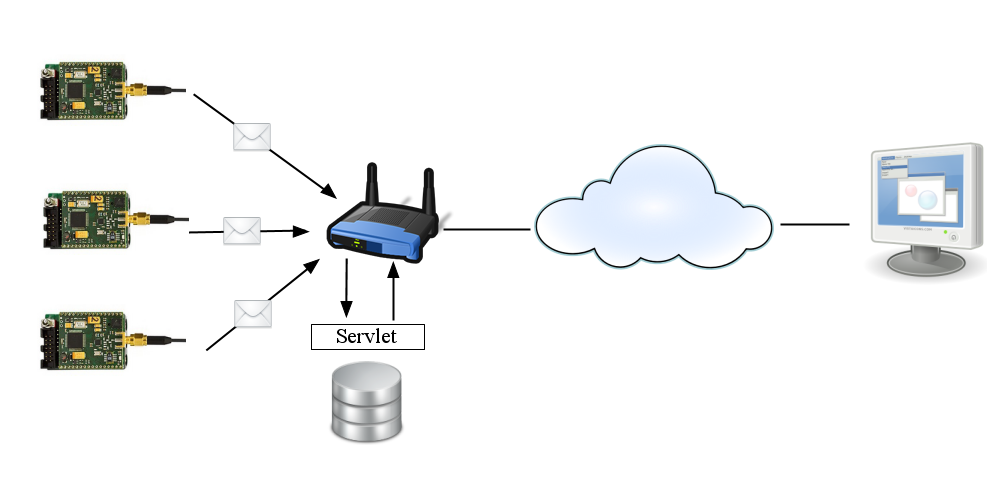
\includegraphics[width=12cm]{fig/Architektur.png}
   \caption{Architektur}
   \label{architecture}
\end{figure}

\subsection*{Modellierung}
Für die Modellierung der Daten wurden folgende Typen identifiziert: 
\begin{itemize}
\item 
\textbf{Property}: Regelmäßig gemessener Wert, wie z.B. Temperatur oder Luftfeuchtigkeit
\item 
\textbf{Trigger}: Vom Benutzer festgelegtes Verhalten beim
Erfüllen einer Bedingung
\item 
\textbf{Event}: Spontanes Ereignis eines Sensors oder eines ausgelöster Trigger
\item 
\textbf{Action}: Aktion die bei einem Event ausgeführt wird
\end{itemize}

\paragraph{Eine Property} beschreibt einen regelmäßig von einem Sensor gemessenen Wert. Der bei diesem Projekt eingesetzte Sensor-Knoten \ref{sec:sensor} misst Temperatur, Luftfeuchtigkeit und Lage im Raum. Das System kann aber leicht auf weitere Properties, wie z.B. Rotation mit einem Gyroskop, oder Koordinaten eines GPS-Senders erweitert werden. 
\paragraph{Ein Trigger} definiert eine Regel, die auf Properties angewandt wird. Z.B. Überschreitung oder Unterschreitung eines Messwertes. Diese Trigger wurden in dem Software-System implementiert. Weitere Trigger könnten Vergleiche auf bestimmte Referenzwerte sein, Zeitabstand der Messwerte, Bereichs-Überprüfung, Auswertung mit komplizierteren Formeln, Anwendung von (Kalman-)Filtern  und vieles mehr. 
\paragraph{Ein Event} beschreibt ein Vorkommnis eines bestimmten Event-Typs zu einem  Zeitpunkt. Ein Event-Typ kann ein Knopfdruck am Sensor oder aber das Auslösen eines Triggers sein. Dabei kann ein Trigger auch viele verschiedene Event-Typen auslösen. Weitere Event-Typen, die in diesem Projekt aber nicht implementiert wurden, sind z.B. Zeit-Ticks, Events von externen Generatoren (SMS, Mail, ...) oder manuelles Erstellen eines Events durch einen Benutzer.

\paragraph{Eine Action} besteht aus Programm-Code, welcher ausgeführt wird, sobald ein Event eintritt. Diese Actions können weitere Events generieren, den Benutzer benachrichtigen oder beliebige Aktionen durchführen. Dabei kann zwischen Actions unterschieden werden, welche auf dem Server ausgeführt werden oder aber beim Client im Browser. In diesem Projekt wurden zu Demonstrationszwecken zwei Aktionen implementiert: Zum einen eine serverseitige Konsolen-Benachrichtigung, zum anderen ein Dialogfenster, welches beim Client im Browser angezeigt wird. 

\section{Verwendetet Technologien} \labelSec{abschnitt}
\subsection{Linux Voyage \cite{voyage}} 
Als Betriebssystem für unseren Access Point haben wir uns für Linux Voyage entschieden. Linux Voyage ist eine abgespeckte Version von Linux Debian, die für Access Points, Asterisk/VoIP Gateways und ähnliche Geräte geschrieben wurde. Da wir auf dem Access Point eine Flashkarte von 8 GB zur Verfügung hatten, war dieses Betriebssystem aufgrund seiner geringen Größe von 128MB besonders gut geeignet. Des weiteren sind alle wichtigen Treiber schon enthalten, sodass wir diese für die WLAN Karte lediglich aktivieren mussten. \\
Ein weiterer Vorteil ist, dass weitere Software wie gewohnt über die Konsole installiert werden kann. So konnten wir ohne weitere Umstände eine MySQL-Datenbank und den Tomcat-Webserver installieren.

\subsection{GWT}
Google Web Toolkit ist ein Toolkit zur Entwicklung und Optimierung von Browser-basierten Anwendungen \cite{gwt}. Der Code wird dabei vom Entwickler in Java geschrieben und anschließend vom GWT-Compiler in Javascript-Code umgewandelt. \\
Die Vorteile bei GWT sind:
\begin{itemize}
 \item Browser-Kompatibilität
 \item Testen in Java (Unit-Tests sind auch möglich)
 \item Entwickler benötigt keine Javascript Kenntnisse, da der Code in Java geschrieben wird
 \item viele Zusatz-Frameworks (z.B. Smart GWT)
 \item umfangreiche Dokumentation und Beispielanwendungen
\end{itemize}

Man muss allerdings erst den Aufbau von GWT verstehen, was am Anfang sehr aufwendig sein kann. So ist dieses Framework nicht unbedingt bei kleinen Anwendung zu empfehlen. \\
GWT war für unser Projekt sehr hilfreich, da die Webseite abhängig von dem Backend aufgebaut wurde und durch GWT-RPC eine einfache Anbindung an das Backend gegeben war.\\
\newline
Im Rahmen dieses Projektes wurde GWT als Plugin für Eclipse \cite{gwtplugin} verwendet.

\subsection{Smart GWT}
Smart GWT ist ein Framework, welches, basierend auf GWT, eine Vielzahl von Erweiterungen der graphischen Oberfläche anbietet. Da es viele Widgets enthält, die GWT nicht besitzt, wurde es für dieses Projekt verwendet.\\
Dabei bietet Smart GWT über die Showcases \cite{smartgwt} viele Codeschnipsel, welche die Entwicklung einfach gestalten. Des weiteren lässt sich Smart GWT sehr leicht in ein GWT-Projekt einbinden. Der Nutzer lädt lediglich Jar-Archive herunter, die eingebunden werden müssen. \\
Der Nachteil von Smart GWT ist allerdings, dass man die Komponenten nicht mit Komponenten von GWT kombinieren sollte (also zum Beispiel sollte man keine Smart GWT Buttons in Layouts von GWT involvieren), da dies zu unerwarteten Effekten führen kann.\\
\newline
Möchte man Smart GWT nutzen, so muss die Jar-Datei (unter: \cite{smartgwtdown}) heruntergeladen werden und in den „Build Path“ eingebunden werden.\\
In der Datei „*.gwt.xml“ \footnote{steht f"ur den Namen des Web Application Projekts} muss nun noch die folgende Zeile eingefügt werden:

\lstset{language=HTML}
\begin{lstlisting}
<inherits name="com.smartgwt.SmartGwt"/>
\end{lstlisting}

\subsection{Charts von Google}
Google Visualization bietet viele Möglichkeiten, Charts und Tabellen in GWT zu erstellen. Dabei werden die Charts in Javascript geschrieben. Allerdings bietet Google auch ein Jar für GWT-Dateien an, so das an dieser Stelle der Programmierer Java-Code schreiben kann. \\
Um ein Chart zu erstellen, muss der Nutzer lediglich eine Datentabelle (DataTable) von Google erstellen und dabei die Formate der Eingabedaten festlegen. Diese Daten werden dem gewünschten Chart mitgegeben und dieser wird auf der Oberfläche dargestellt. Alles weitere wird mitgeliefert wie zum Beispiel die „Clickevents“, oder die dynamische Größenanpassung der Charts an die Menge der Daten.\\
Aber auch hier ist der Nachteil, dass man Charts von Google nicht einfach mit Smart GWT Elementen kombinieren kann, dafür aber mit GWT Elementen.\\
\newline
Um Google Charts nutzen zu können, muss man die Jar-Datei (unter: \cite{charts}) herunterladen und in das Projekt im „Build Path“ einbinden. In der Datei „*.gwt.xml“ muss nun die folgende Zeile eingefügt werden.
\lstset{language=HTML}
\begin{lstlisting}
<inherits name='com.google.gwt.visualization.Visualization'/>
\end{lstlisting}

\section{Sensor-Knoten} \label{sec:sensor}
Der verwendete Sensor-Knoten basiert auf dem MSB430H-Board. Es enthält mehrere Sensoren. Diese sind der SHT11-Sensor , welcher die Temperatur und Luftfeuchtigkeit misst und der MMA 7260Q G-Sensor, 
mit dem die relative Lage des Sensor-Knotens im Raum festgestellt werden kann. Der Sensor-Knoten wurde mit dem WLAN-Modul RN-134 der Firma Roving Networks über die UART-Schnittstelle fest verlötet. 
Die Kommunikation zwischen dem programmierbaren Board und dem WLAN-Modul erfolgt also über die serielle Schnittstelle. An dieser Schnittstelle wurde ein Kipp-Schalter und  ein serielles Kabel angebracht, 
welche es ermöglichen, den Daten-Austausch zwischen Board und Modul zu verfolgen. Damit fiel das Debuggen der Kommunikation leichter.

\subsection{HTTP-Kommunikation}
\label{ssec:HTTP}
Bei der Erprobung des WLAN-Moduls über eine serielle Schnittstelle haben wir verschiedene Übertragungsverfahren getestet: 

\begin{itemize}
 \item Das Modul bietet die Möglichkeit, alle x Sekunden einen UDP-Broadcast zu senden, welcher die auf dem Modul gesetzte Zeit beinhaltet und alle gemessenen Sensor-Werte. Dies ist für das Projekt nicht praktikabel, da die Sensoren nicht direkt an das WLAN-Modul angeschlossen sind, sondern an dem Sensor-Knoten. Deswegen ist auch der UDP-Unicast unbrauchbar.
 \item Das Modul bietet die Möglichkeit, eine TCP Auto-Connection zu nutzen, also automatisch alle x Sekunden aufzuwachen und eine TCP-Verbindung zu einem vordefinierten Host aufzurufen. Da das WLAN-Modul aber keine Werte vom Sensor-Knoten pollen kann, ist diese Methode ebenfalls unbrauchbar. 
 \item Eine weitere Methode, die aber ebenfalls wegen des oben beschriebenen Grundes fehlschlägt ist das automatische Senden von Sensor-Daten an einen HTTP-Server. 
\end{itemize}

Nach ausgiebigen Tests haben wir uns entschieden, die Daten über eine TCP-Verbindung zu verschicken. Diese wird von dem Sensor-Knoten geöffnet. Danach wird ein GET-Befehl des HTTP-Protokolls (HTTP 1.1) abgesetzt. Dabei wird angegeben, dass die Verbindung nicht geschlossen werden soll. Dies ermöglicht es, mehrere Datensätze hintereinander mit Hilfe des GET-Befehls zu versenden, ohne die TCP-Verbindung jedes Mal neu initiieren zu müssen. Da die Verbindung nach ca. 5 Minuten vom Server geschlossen werden würde, muss sie in regelmäßigen Abständen vom Client geschlossen und direkt danach neu aufgebaut werden.  \\
Das WLAN-Modul verschickt einen festgelegten String (Default: „*HELLO* “) beim erfolgreichen Aufbauen der TCP-Verbindung. Dieser String darf nicht leer sein darf. Das hat uns zuerst Probleme bereitet, da der Tomcat-Server unbekannte Befehls-Präfixe nicht ignoriert. Die Lösung ist das Benutzen von „GET“ als Communication-String. Da dieser aber nur beim Starten der Verbindung gesendet wird, muss jeder weitere GET-Befehl vollständig übertragen werden. Dies ist eine unschöne Lösung, allerdings lies sich das Problem nicht anders beheben, da das WLAN-Modul selbst nicht programmiert werden kann.

\subsection{Konfiguration des WLAN-Moduls}
Bei jedem Start des Sensor-Knotens muss das WLAN-Modul in einen wohldefinierten Zustand gebracht werden. Da beim Booten des Knotens nur schwer verifiziert werden kann, 
ob alle Einstellungen korrekt vorgenommen wurden, haben wir uns dafür entschieden, dass das WLAN-Modul bei jedem Start auf die Fabrikeinstellungen  zurück gesetzt und dann neu konfiguriert wird. 
Dies ist nötig, da beim Programmieren der Sensor-Knoten zwar neu gestartet, beim Debuggen die Stromversorgung des WLAN-Moduls aber nicht unterbrochen wurde und es so in einem beliebigen Zustand sein könnte. 
Das Zurücksetzen hat ebenfalls den Vorteil, dass das Modul nicht vor dem ersten Betrieb explizit initiiert werden muss, allerdings dauert jeder Boot-Vorgang etwas länger. Insgesamt jedoch werden bereits ca. 10 Sekunden nach dem Einschalten die ersten Sensor-Werte gesendet. 


\subsection{Programmierung des Sensor-Knotens}
Für die Programmierung des Sensor-Knotens wurde der Code Composer Essentials Professional (Version: CCE v3.1, Build: 3.2.4.3.8)  verwendet. Die Programmiersprache ist ein C-Dialekt, welcher fast alle Funktionen des Standards bereit stellt. \\
Das Programm des Sensor-Knotens besteht aus zwei Teilen: Zuerst wird eine Initalisierungs-Phase durchlaufen in der Interrupts angeschaltet werden, nötiger Speicher alloziert und das WLAN-Modul konfiguriert wird. Danach beginnt eine Endlos-Schleife, die das Betriebssystem darstellt. 
In dieser Schleife werden die Sensor-Werte ermittelt und dann per WLAN verschickt.

\subsubsection{Initialisierung}
Bei der Initialisierung werden folgende Schritte chronologisch ausgeführt: 

\begin{itemize}
 \item Initialisierung der Port Register
 \item Aktivierung der quarzstabilen XT2 Taktquelle (7.3728MHz)
 \item Initialisierung der UART-RS232 Schnittstelle mit 9.6kBit/s
 \item Einschalten der Interrupts für die beiden Taster, Freigeben der Interrupts und  Aktivierung der Interrupt-Routinen
 \item Zurücksetzen des WLAN-Moduls in den Auslieferungszustand
 \item Setzen von WLAN-SSID, Passwort und anderen Parametern
 \item Verbindungsaufbau mit dem Access Point und einrichten der TCP-Verbindung zum Tomcat-Server
\end{itemize}
Dann tritt das System in die zweite Phase ein.

\subsubsection{Betriebssystem}

Das „Betriebssystem“ besteht aus einer Endlos-Schleife, in der folgende Aktionen ausgeführt werden:
\begin{itemize}
 \item Überprüfung, ob bereits 20 Abfragen gesendet wurden; ggf. Trennung und erneuter Aufbau der TCP-Verbindung (der Server würde die Verbindung nach ca. 5 Minuten trennen)
 \item Auslesen der Sensoren, Aufbereitung der gelesenen Werte und Speicherung des Requests in einer Warteschlange, welche alle zu sendenden GET-Anfragen enthält
 \item Falls die Verbindung nicht gerade neu geöffnet wurde, wird „GET “ dem Request voran gestellt (Grund siehe Abschnitt \ref{ssec:HTTP})
 \item Solange noch weitere Requests in der Warteschlange sind, werden diese ebenfalls entfernt und dann versendet
\end{itemize}

\subsubsection{Tastendruck}
Die Erkennung eines Tastendrucks geschieht in dem Interrupt, welcher in der Initialisierung definiert wurde. Dort wird direkt beim Interrupt und 0.5 Sekunden nach dem Auslösen gemessen, welcher Taster gedrückt wurde und dann beide Messungen logisch verodert. Damit können wir mit einem Interrupt ebenfalls feststellen, ob beide Taster gleichzeitig gedrückt wurden. Weiterhin kann damit ausgeschlossen werden, dass die analog gemessene Größe am Anfang noch etwas flackert und eventuell beim ersten Auslesen den falschen Wert liefert. Danach wird ein GET-Request für das Taster-Event erstellt und in die Warteschlange eingereiht. Beim nächsten Durchlauf der Betriebssystem-Schleife wird dieser Request dann ebenfalls mit verschickt. Die Auflösung der Tasten-Events ist damit gleich einem Schleifendurchlauf, der bei durchschnittlich 3 Sekunden, maximal bei 7 Sekunden (Trennen und neuer Aufbau der Verbindung) liegt. 

\section{Backend}\label{sec:backend}
Das Backend des Projekts nimmt die von Sensoren gemessenen Größen entgegen, verarbeitet diese Daten vor, speichert sie und stellt diese Daten zur Verfügung. Das Backend ist in zwei Teile aufgeteilt. Im ersten Teil des Kapitels wird auf die Daten-Verarbeitung eingegangen, welche in einem Java-Servlet auf dem Tomcat-Server läuft, danach auf die Bereitstellung der Daten für das GWT-Frontend \ref{sec:frontend} mittels GWT-RPC.

\subsection{Datenbank-Zugriff}
Um bequemen Zugriff auf die Datenbank zu erhalten, benutzen wir spezielle Proxy-Klassen, welche die MySQL-Datenbank in Klassen abstrahiert. Damit wir diese Klassen nicht selbst schreiben mussten (das dazugehörige Entwurfsmuster heißt DAO - DataAccessObjects in Kombination mit DTO - DataTransferObjects), haben wir einen DAO-Generator benutzt, welcher ein gegebenes SQL-Schema interpretiert und dann daraus Java-Klassen generiert. Der Generator, den wir benutzt haben, heißt FireStormDAO 4.0.1.

\subsection{Daten-Verarbeitung}
Die Daten-Verarbeitung besteht aus drei Dingen : 
\paragraph{Bei der Auswertung der HTTP-GET-Requests} wird zuerst der Typ der gesendeten Daten überprüft. Dieser Typ ist in dem Parameter \textit{action} gespeichert. Anhand dieses Parameters wird dann entschieden, welche Methode zur Verarbeitung aufgerufen wird. Im Moment gibt es zwei zuständige Methoden: doKeyEvent und doProperty (Die Namensgebung orientiert sich an dem Servlet-Interface).\\
Die doKeyEvent-Methode speichert den Zeitpunkt des Events zusammen mit dem gedrückten Knopf (1: schwarz, 2: gelb, 3: beide) in der Datenbank ab. Danach wird die handleEvent-Methode zur Abarbeitung eventueller Aktionen bei einem Key-Event aufgerufen (s.u.). \\
Die doProperty-Methode extrahiert die gemessenen Werte aus dem GET-Request. Im Moment sind diese Werte Temperatur, Feuchtigkeit und Lage im Raum (2 Werte). Zuerst müssen die Werte erneut gerundet werden, da die Floating-Point-Unit des Sensor-Knotens nicht besonders genau ist. Dann wird jeder einzelne Wert mit Zeitstempel und einer Referenz auf den sendenden Knoten in der Datenbank abgelegt. 

\paragraph{Die Event-Erkennung} wird direkt im Anschluss gestartet. Hierbei werden die Trigger für den entsprechenden Sensor-Knoten und die dazugehörige Property geladen und dann verglichen, ob die Property den definierten Schwellwert $s$ des Triggers überschreitet. Abbildung \ref{event-detection} verdeutlicht unseren Mechanismus: Der im Trigger definierte Wert von 30°C (schwarze Linie) wurde überschritten. Bei der Ankunft des ersten gemessenen Wertes, der $s$ übertrifft, wird vom Backend ein Start-Event generiert. Dieses bedeutet, dass der Schwellwert überschritten wurde. Damit ein Zittern um den Schwellwert herum ausgeschlossen werden kann, haben wir einen zweiten Schwellwert eingestellt (rote Linie). Dieser liegt um $\Delta$ verschoben in Richtung des normalen Wertebereiches, also bei einem Trigger für Wert-Überschreitung bei $s - \Delta$.
Wird dieser zweite Schwellwert wieder unterschritten, so wird ein Stop-Event generiert. 

\begin{figure}[htbp]
   \centering
   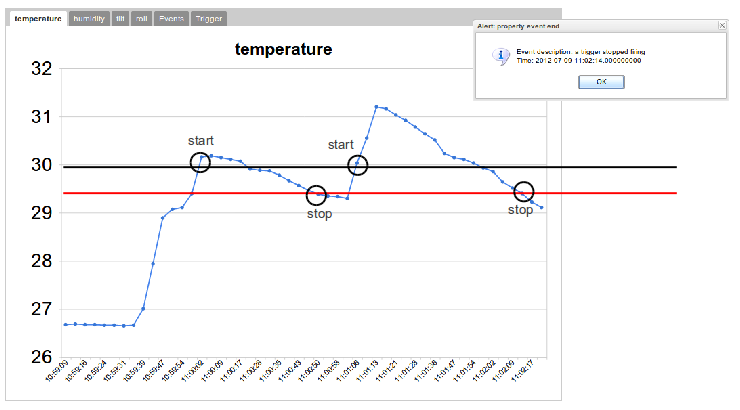
\includegraphics[width=12cm]{fig/threshold.png}
   \caption{Event-Erkennung mit Thresholds}
   \label{event-detection}
\end{figure}
\missingfigure{die Grafik sollte neu gemacht, das Delta hinzugefügt und in höherer auflösung gespeichert werden }

\paragraph{Das Event-Handling} wird nach jeder Event-Generation gestartet. Dabei wird überprüft, welche Actions für diesen Event-Typ registriert sind und führt diese aus. Es wird zwischen serverseitigen Aktionen und clientseitigen Aktionen unterschieden. Damit könnte das System mit anderen Komponenten gekoppelt werden, z.B. eine Benachrichtigung per SMS, E-Mail oder eben ein clientseitiger Alarm/Notifikation.

\subsection{Daten-Bereitstellung}Die Daten-Bereitstellung für das Frontend geschieht mit GWT-RPC. Eine genauere Erklärung findet sich in Abschnitt \ref{ssec:aufbau}. Die bereitgestellten Methoden dienen der Abfrage der Datenbank und lassen außerdem Manipulationen zu. Hier wird starker Gebrauch von den DataAccessObjects gemacht.

\section{Frontend}\label{sec:frontend}
Die Sensoren, die im Haushalt verteilt sind, schicken die gemessenen Daten an den Access Point. Nun müssen diese Daten in geeigneter Weise aufbereitet und dem Nutzer zur Verfügung gestellt werden. Hierfür wurde ein web-basiertes Frontend gebaut, welches die gemessenen Daten in Diagrammen darstellt. \\
In diesem Kapitel wird dieses Frontend vorgestellt und beschrieben.

\subsection{Anforderungen}

An die Webseite, die es dem Nutzer ermöglicht, die Daten der Sensoren zu überwachen, gibt es eine Reihe von Anforderungen. \\
Eine wichtige Anforderung ist die benutzerfreundliche Oberfläche, welche einfach gehalten werden soll um so dem Anwender zu ermöglichen, sich schnell einzuarbeiten. Aus diesem Grund wurde die Oberfläche sehr schlicht gehalten und auf das Wesentliche reduziert.\\
Über eine Drop-down-Box kann der Nutzer zwischen den verschiedenen Sensoren auswählen und sich Daten anzeigen lassen. Dabei wird ein Diagramm für jede gemessene Property angezeigt. In unseren Fall hatten wir also ein Diagramm für die Temperatur, Feuchtigkeit und 2 Diagramme für die Neigung des Sensors. Da es aber möglich sein soll, andere Sensoren an das System anzuschließen, welche andere Daten (Propertries) messen, passt sich die Oberfläche mit den Diagrammen an die jeweiligen Daten an.\\
Nun kann der Nutzer die gemessene Werte überwachen. Die Diagramme werden in Echtzeit aktualisiert. Dabei hat der Benutzer aber nur ein Diagramm gleichzeitig im Blick, da pro Diagramm ein Tab in einem Tab-Menü zur Verfügung steht. Es kann passieren, dass der Anwender so zum Beispiel nicht beobachten kann, dass die Temperatur im Kühlschrank stetig zunimmt, weil er das Diagramm mit der Neigung des Sensors geöffnet hat. Damit der Nutzer trotzdem gewarnt wird, wurden Trigger in unser System integriert. Wird ein Trigger ausgelöst, so erscheint eine Dialogbox auf der Webseite und eine System-Ausgabe wird auf der Konsole des Servers ausgegeben.\\
Eine weitere Anforderung an das System war es, dass der Standort eines Sensors bearbeitet werden kann und dieser dann in die Datenbank abgespeichert wird. Es kann passieren, dass der mobile Sensorknoten an einen anderen Ort platziert wird. Bei der Anzeige der Sensordaten kann der Benutzer auf „Edit“ klicken und den Ort des Sensors bearbeiten. Die ID und die IP sollen nicht geändert werden. \\
Alle diese Anforderungen sind für die leichte Bedienbarkeit der Oberfläche und wurden in diesem System umgesetzt.

\subsection{Projektaufbau}
\label{ssec:aufbau}
Da für dieses Projekt GWT genutzt wurde, war der Aufbau des Frontends zum Teil durch die Struktur von GWT vorgegeben. \\
In dem Package „src/de/berlin/fu/client“ befindet sich die Datei „TelproGWT.java“ in der man den Hauptteil des Frontends findet. In der Datei „TelproGWT.gwt.xml“ im Package „src/de/berlin/fu/berlin“ wird definiert, welche onModuleLoad-Methode welcher Klasse (in unserem Fall TeproGWT) aufgerufen werden soll. \\
Ein wichtiges Interface in diesem Projekt ist das Service-Interface „MyServer.java“, welches sich in dem Ordner „src/de/berlin/fu/shared“ findet. Dieses gibt vor, welche Methoden von der Clientseite genutzt werden können um mit dem Backend zu kommunizieren. Damit nun die Clientseite die Methoden der Serverseite nutzen kann, muss ein sogenanntes Async-Interface erstellt werden. Dieses befindet sich auch in dem Ordner „src/de/berlin/fu/shared“ und heißt „MyServerAsync.java“. Es wird ein asynchrones Interface definiert, da man vermeiden möchte, dass die Web-Anwendung beim Aufruf der Methoden der Serverseite einfriert und der Anwender warten muss. Google Web Toolkit gibt diese Art von Interface bei GWT-RPC immer vor. In der Klasse, welche die Benutzeroberfläche implementiert, wird dieses Async-Interface initialisiert. 
In den anderen Packages befindet sich die Implementation der Backendseite, welche in dem Kapitel \ref{sec:backend} näher erläutert wird.


\subsection{Code}
Die Klasse TelproGWT.java ist die Klasse, in welcher der clientseitige Code steht. Jede Klasse in GWT, welche den Client-Code enthält, muss das Interface „EntryPoint“ implementieren. Dabei wird von GWT vorgeschrieben, dass die Methode „onModuleLoad“ überschrieben werden muss. Diese Methode wird aufrufen, sobald der Anwender die Webseite in dem Browser aufruft.\\
Wird die onModuleLoad-Methode aufgerufen, holt sich die Clientseite als erstes alle Propertytypen und Eventtypen die in der Datenbank abgespeichert wurden über einen entsprechenden RPC-Call. Diese Typen werden an mehreren Stelle im Programm benötigt. Um nicht mehre Datenbankanfragen und somit die Anwendung langsamer zu machen, werden die Typen beim Laden der Webseite abgefragt und in einer HashMap abgespeichert. \\
Mit den Propertytyen kann nun dynamisch die Ansicht für die Liniendiagramme aufgebaut werden. Pro Propertytyp wird ein Tab mit einem Liniendiagramm aufgebaut und in das Tab-Menü eingepflegt. Dieses Tab-Menü ermöglicht es, dass nur das Diagramm aktualisiert werden muss, welches gerade angezeigt wird. Dieser Schritt war nötig, da das angezeigte Diagramm möglichst oft aktualisiert werden soll (alle 3 Sekunden) und sonst der Datenverkehr zu hoch und die Performance der Anwedung zu niedrig wäre.\\
Die Events werden in den 3 Sekunden immer mit aktualisiert und es ist egal, ob der Nutzer sich die Eventtabelle ansieht oder nicht. Löst ein Event nun eine Aktion aus, so soll der Anwender informiert werden (zum Beispiel über ein Dialogfenster), wenn dieses eintritt. So erhält man ein Warnsystem, welche wichtig für dieses System ist.\\
Durch GWT können nicht nur Oberflächenelemente eingefügt werden, sondern auch gestaltet werden. Zum Beispiel kann die Größe, Farbe, der Rahmen und vieles mehr verändert werden. Wie die Oberfläche aussieht, kann dem nächsten Abschnitt und den darin enthaltenden Bildern entnommen werden.

\subsection{Screenshots}

Um einen Überblick über das Interface zu bekommen, werden hier einige Screenshots gezeigt.   
\begin{description}
\item[Abbildung \ref{screen1}:] Auswahl der Sensoren in einer Drop-down-Box. 
\item[Abbildung \ref{screen2}:] Wurde ein Sensor ausgewählt, wird diese Ansicht angezeigt. Oben rechts befinden sich die Sensorinformationen, welche man bearbeiten kann. In der Mitte findet man die Einstellungsmöglichkeiten für Ansicht der Diagramme. Zum einen kann die Anzahl der Daten-Punkte in dem Diagramm eingestellt werden, zum anderen die Skalierung der X-Achse („spreading-factor“).
\item[Abbildung \ref{screen3}:] Das ist die Eventlisten-Ansicht. Die Einstellungsmöglichkeiten für die Diagramme sind ausgestellt.
\item[Abbildung \ref{screen4}:] Diese Ansicht wird gezeigt, wenn der Nutzer auf „Bearbeiten“ des Sensorknotens klickt. Der Ort des Sensors kann bearbeitet werden, die IP und die ID allerdings nicht.
\end{description}

\begin{figure}[h!]
   \centering
   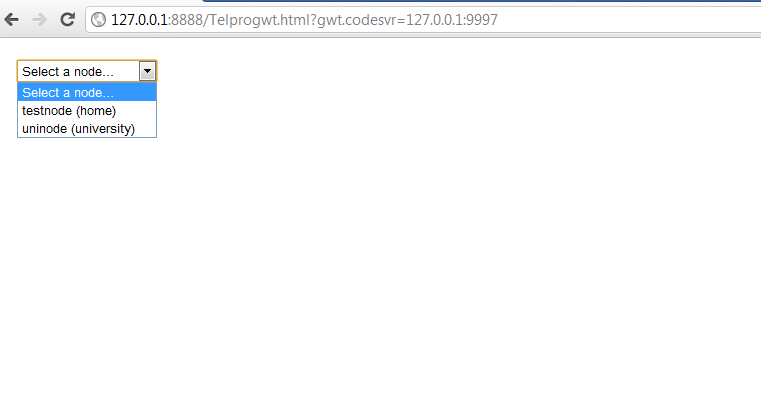
\includegraphics[width=12cm]{fig/screen1.png}
   \caption{Screenshot Drop-down-Box}
   \label{screen1}
\end{figure}

\begin{figure}[h!]
   \centering
   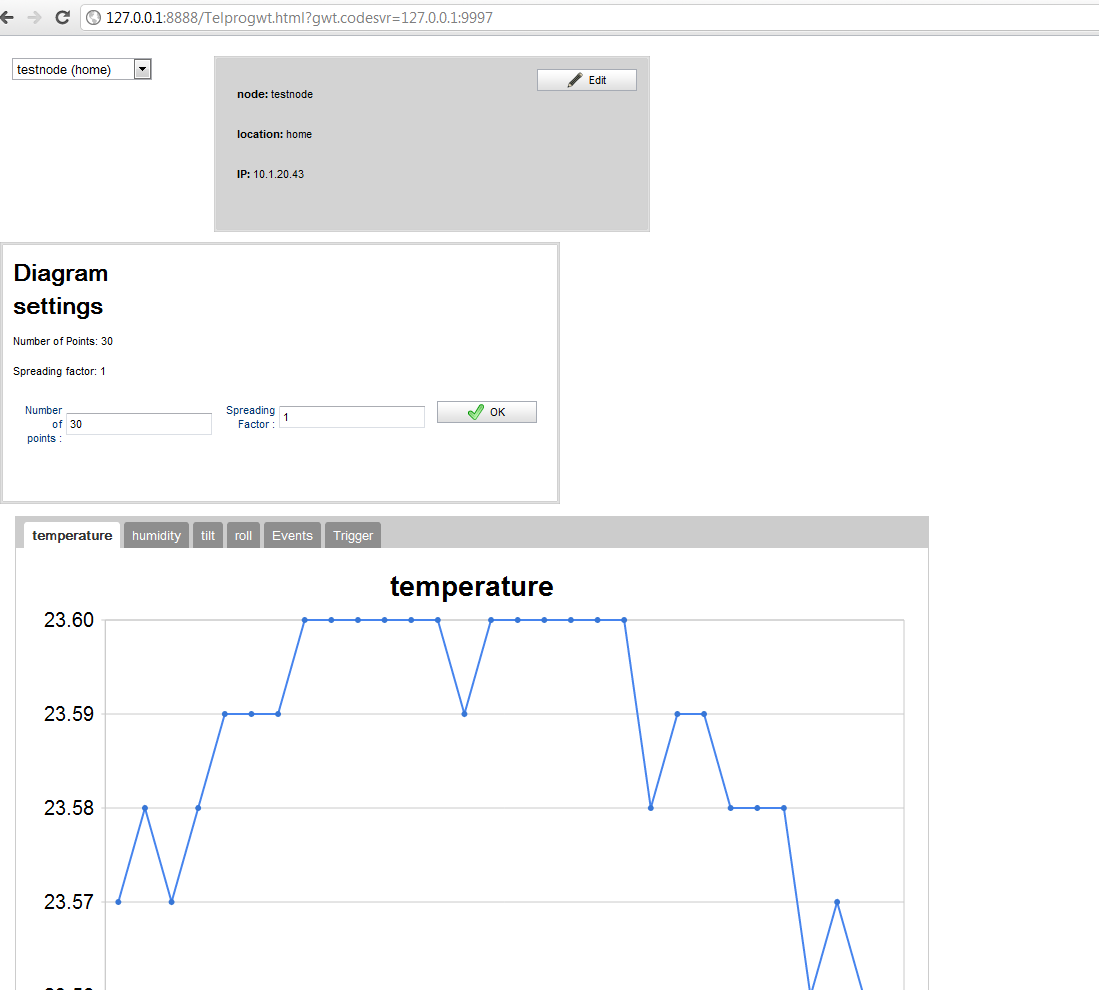
\includegraphics[width=12cm]{fig/screen2.png}
   \caption{Screenshot Hauptansicht}
   \label{screen2}
\end{figure}

\begin{figure}[h!]
   \centering
   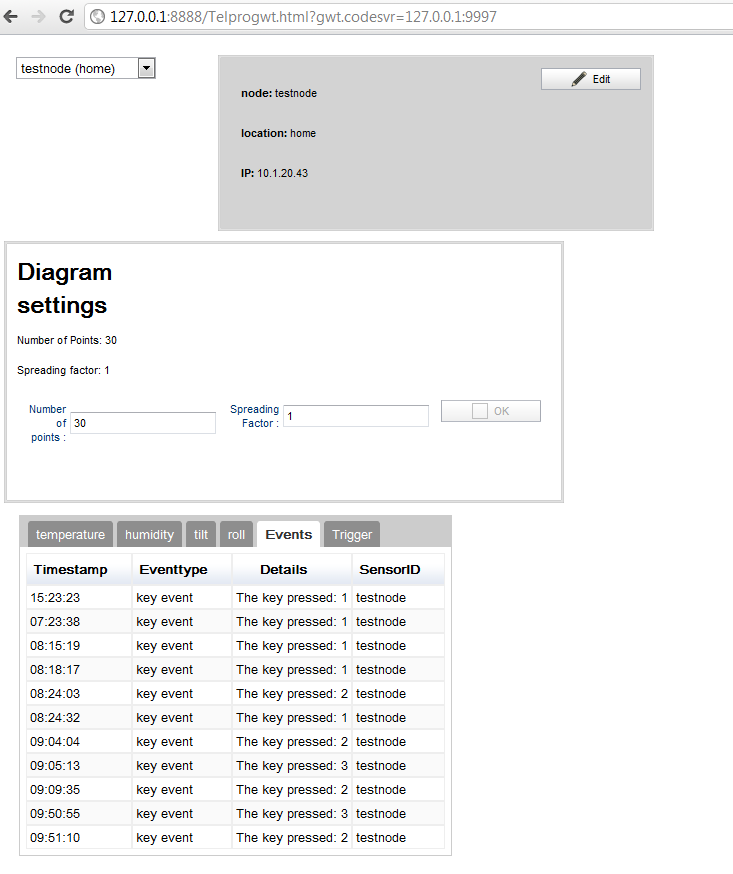
\includegraphics[width=12cm]{fig/screen3.png}
   \caption{Screenshot Eventlisten-Ansicht}
   \label{screen3}
\end{figure}

\begin{figure}[h!]
   \centering
   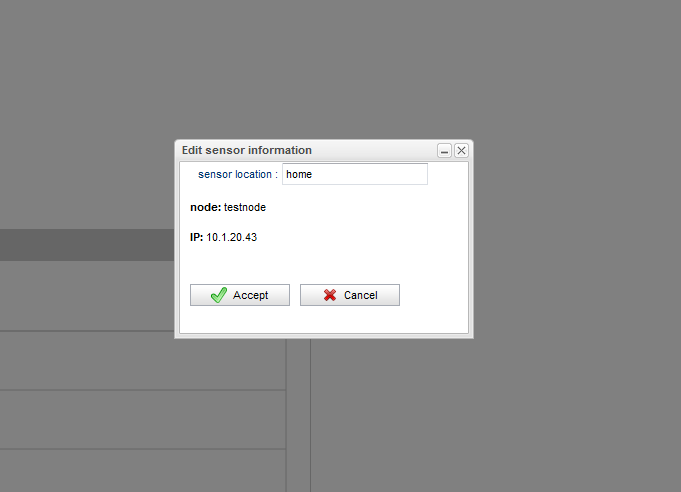
\includegraphics[width=12cm]{fig/screen4.png}
   \caption{Screenshot „Bearbeiten“}
   \label{screen4}
\end{figure}
  
\section{Zusammenfassung und Ausblick} \labelSec{ausblick}
Ziel dieses Projektes war es, sich mit verschiedenen Technologien zu befassen und verschiedene Ebenen der Programmierung zu benutzen. Wir haben Konzepte von administrativen Tätigkeiten, wie MySQL-Datenbanken, Linux und Tomcat-Servern, über die hardwarenahe Programmierung und Arbeit mit externen Hardware-Modulen (WLAN) bis hin zu hochsprachigen Web-Plattformen, welche viele Dinge abstrahieren, aber auch neue Schwierigkeiten bereiten, erlernt und zum ersten Mal viele kleine Systeme zu einem großen Ganzen zusammengefügt. Der entstandene Prototyp ist so sicher nicht praktikabel, allerdings haben wir so weit, wie möglich, die Erweiterbarkeit in den Vordergrund gestellt, sodass es leicht zu einem simplen Home-Automatisation-Framework werden kann. Wir haben im Verlauf des Projekts viele Erfahrungen gesammelt, von denen wir einige hier beschreiben wollen.
\subsection{Erfahrungen}

\paragraph{Tomcat Webserver}
Die Benutzung und Konfiguration von Appache Tomcat Webserver ist sehr aufwendig und nicht sehr intuitiv. Wir haben sehr viel Zeit damit verbracht, alle Einstellungen vorzunehmen und danach unser Projekt als War-Archiv zu installieren. Diesen Installations-Vorgang mussten wir mehrfach wiederholen, weil manche Dateien nicht aktualisiert wurden. Wie genau der Deployment-Vorgang funktioniert, ist uns bis heute nicht klar. Wir empfinden großen Respekt für die Administratoren, die alle Parameter solcher Programme kennen und genau wissen, wie dieses gigantische Stück Software funktioniert. 

\paragraph{Hardwarenahe Programmierung}
Die Programmierung des Sensor-Knotens war ebenfalls sehr zeitaufwendig. Aufgrund unzureichender Kenntnisse über die Funktionsweise von Mikrocontrollern, ist es uns zunächst schwer gefallen, genau zu durchschauen, was passiert. Man muss seine (Java-)Denkweise komplett umstellen: Es ist nur sehr wenig Speicher vorhanden, man muss nicht objekt-orientiert programmieren und es sind so gut, wie keine Abstraktionen vorhanden. Nachdem die ersten Schritte aber gemeistert waren, konnten wir doch recht gut nachvollziehen, was auf dem Controller-Board passiert und dem entsprechend programmieren.
\subsection{Erweiterungen}
Abschließend wollen wir aufzeigen, welche Erweiterungen interessant für das System wären. Teilweise wurden diese schon im Abschnitt \ref{architecture} aufgezeigt. \\
Weitere 
android app (mit push notifications)
befehle an Sensor senden
\todo{teilweise siehe architektur, sonst blablabla}

\clearpage

\section{Appendix}

% @SETTINGS: Insert the name of your bibliography file WITHOUT extension.
\bibliography{main}

\bibliographystyle{abbrv}

\end{document}
